\chapter{Comparing $\delta$-electrons flagging algorithms}\label{delta}
\textit{In the context of DAQ testing and performance analysis during Mu2e data-taking, 
where the data volume is expected to reach approximately 7 PBytes per year, optimizing 
memory usage and minimizing CPU consumption is crucial. The primary source of hits in the 
Mu2e tracker will be $\delta$-electrons. Therefore, it is essential to effectively flag these 
hits without compromising the efficiency of CE hit detection and track reconstruction. This 
Chapter presents a comparison between two algorithms designed for $\delta$-electron flagging.}
\section{$\delta$-electrons background in Mu2e}
One of the central challenges of the Mu2e experiment is the reconstruction of 
conversion electrons in the presence of significant background noise from 
other processes associated with muon capture by aluminum atoms.

The primary aim of this study is to address one prevalent source of 
background: secondary ionized electrons, known as $\delta$-electrons. 
These electrons primarily consist of Compton scattered electrons, pair production 
electrons, and delta rays, listed in decreasing order of prevalence. Compton 
scattered electrons are generated when photons, produced by various processes, 
interact with the detector material. These photons primarily originate from 
neutron capture by atoms, which excites the nucleus, leading to photon emission 
during decay. Typically, these photons have energies of a few MeV. The neutrons 
are produced when muons are captured by atoms, resulting in unstable isotopes that 
decay by emitting neutrons. Pair production electrons are generated during nuclear 
recoil processes, where pairs of electrons and positrons are produced to conserve 
energy and momentum. Delta rays, or secondary ionized electrons, are generated when 
high-energy charged particles collide with the detector material.

A delta electron is defined as having a momentum below 20 MeV/c; for instance, an 
electron with a momentum of 10 MeV/c would have a radius of less than 3 cm in the 
Mu2e magnetic field. These electrons typically produce a distinctive pattern in the 
Mu2e tracker, often resulting in multiple hits with nearly identical $(x, y)$ coordinates.

In the Mu2e experiment, low-energy electrons constitute about 75\% of the tracker hits, 
making their management crucial for memory efficiency. These hits can also interfere with 
track reconstruction, necessitating their precise identification and filtering to preserve 
data accuracy. It's essential to correctly identify these hits to prevent misidentification 
of conversion electrons and to accurately estimate the muon stopping rate, which in turn 
requires proper identification of protons. Additionally, distinguishing between background 
sources like low-energy electrons and positrons, and the hits from muons and pions, is 
critical to maintain the integrity of the analysis and the accuracy of background estimation.

\section{Mu2e $\delta$-electrons rejection algorithms}
The $\delta$-electrons flagging is a stage of Mu2e reconstruction tool that comes 
before the time cluster and the pattern recognition.
The Mu2e Offline software tool is illustrated in Appendix \ref{mu2eana} and 
the reconstruction process is described in Appendix \ref{eventreco}.
In Mu2e Offline, there are two different types of rejection algorithms:
\begin{itemize}
    \item DeltaFinder;
    \item FlagBkgHits.
\end{itemize}
\begin{figure}[!h]
    \begin{subfigure}[b]{0.4\linewidth}
        \centering
        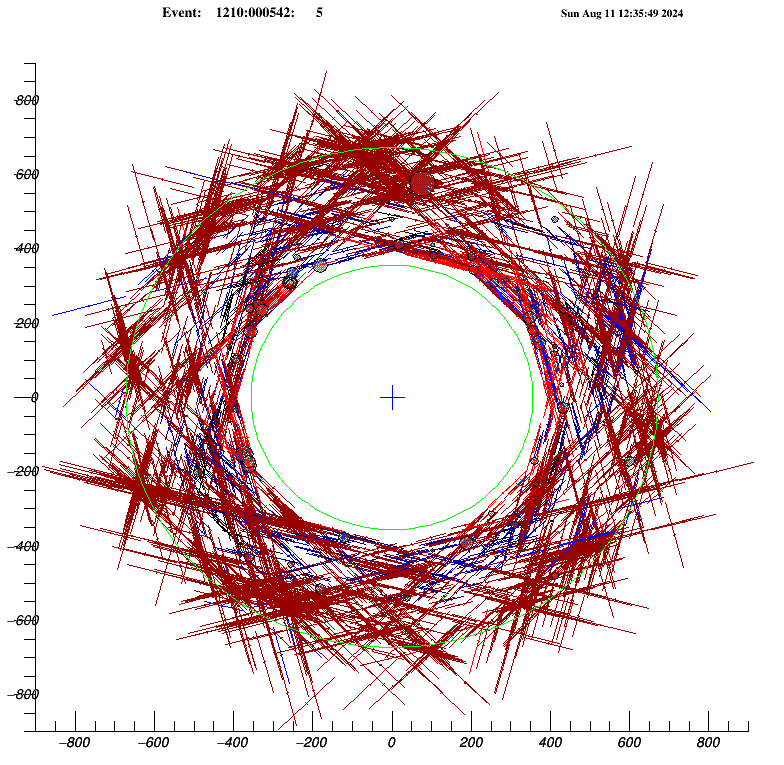
\includegraphics[scale = 0.3]{figures/png/Screenshot_20240811_123612.png}
        \subcaption{Before.}
        \label{fig:bef}
    \end{subfigure}
    \begin{subfigure}[b]{0.7\linewidth}
        \centering
        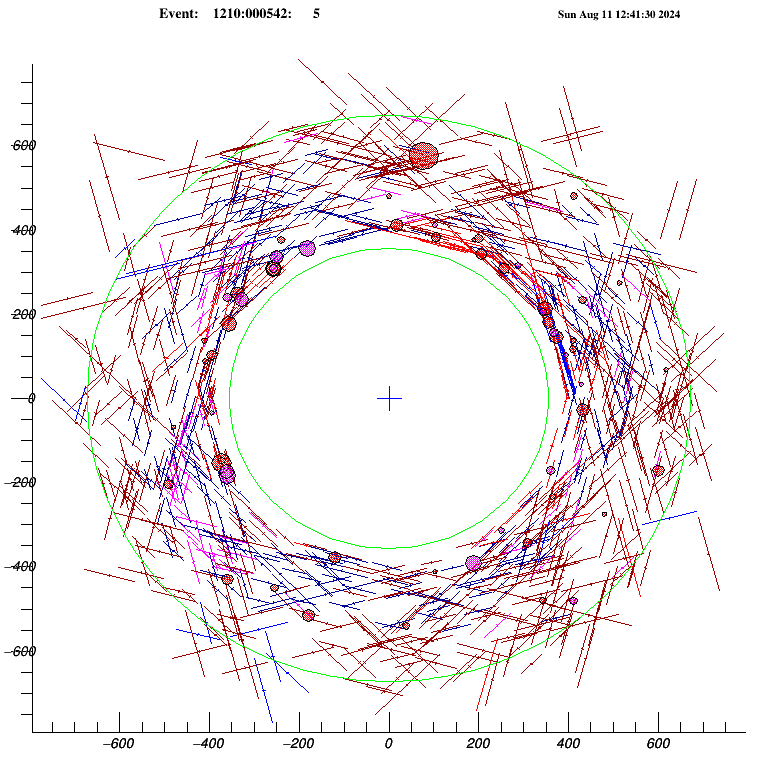
\includegraphics[scale = 0.3]{figures/png/Screenshot_20240811_124245.png}
        \subcaption{After.}
        \label{fig:af}
    \end{subfigure}
    \caption[Before and After background hits flagging.]{Before and After background hits flagging. 
    The transverse $x-y$ views of a CE event 
    with 2BB pile-up (Section \ref{pulsedprotonbeam}). The segments are the tracker $StrawHit$s. The hits marked in
    dark red are from low energy electrons and the ones in blue are from positrons.}
       \label{fig:befaf}
\end{figure}
\subsubsection{$FlagBkgHits$ Algorithm}
flgbkg flags hits with high charge
The description of a multivariate analysis is outside the scope of this work and so is the process
of MVA-training. Since these techniques are fundamental for the background flagging, we will briefly
describe the basic principles. When looking for patterns in a multi-variable space, it is a common
procedure to define a set of statistical models that examine the variables measured and estimate the
probability that these are compatible with the pattern. Once the variables have been chosen, the
MVA is trained to recognize patterns by looking at examples known to the trainer and a feedback can
be provided to improve the identification.
When looking for $\delta$-electrons, the most significant variables are the position and spread of the Com-
boHit, both in the XY plane and in the Z direction.

This algorithm 
clusters hits in time and in the $xy$ plane, using 
Multivariate Analysis to distinguish low-energy 
hits from conversion electron hits, which are 
stored for subsequent pattern recognition.
\subsubsection{$DeltaFinder$ Algorithm}
DeltaFinder is an algorithm designed to identify $\delta$-electron hit patterns 
rather than CE hits. This algorithm relies on the fact that $\delta$-electrons usually 
form a straight line in the $r-z$ plane (Figure \ref{fig:yzviewdelta}) and appear as a spot in the $x-y$ plane, 
while CE hits create entirely different patterns. The goal of DeltaFinder is to recognize 
$\delta$ electrons in the Mu2e tracker with high efficiency, minimizing false positives. 
In the process, all hits associated with detected objects are treated as $\delta$-electron hits.
\begin{figure}[!h]
    \centering
    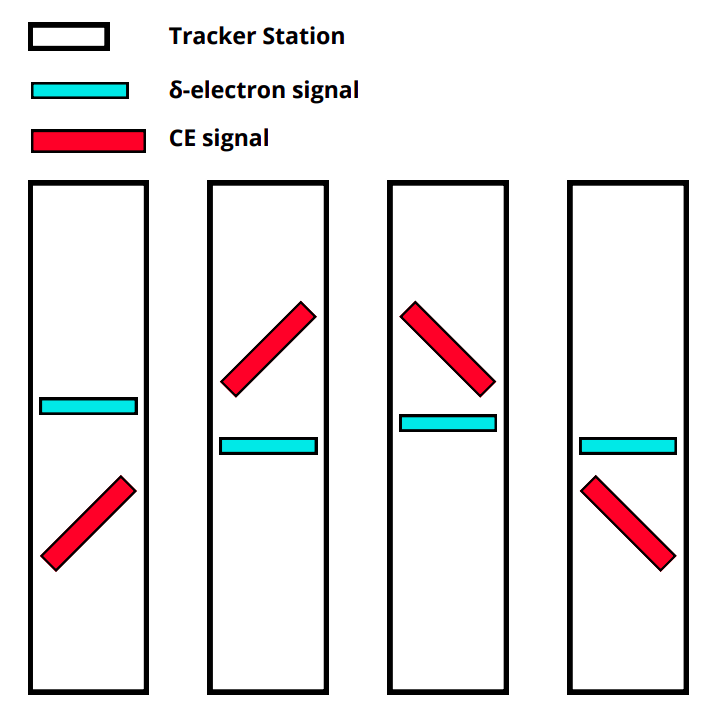
\includegraphics[width =0.6\textwidth]{figures/png/Screenshot_20240811_123048.png}
    \caption[$\delta$-electrons $y-z$ plane pattern.]{    }
    \label{fig:yzviewdelta}
\end{figure}
\paragraph{Step 1: Identifying $\delta$-Electron Segments}

DeltaFinder first identifies $\delta$-electron track segments within 
each station separately. $\delta$-electron hits, which may occur in multiple 
straws within the same tracker panel, are clustered in space-time. The algorithm 
performs several cleanup cuts to ensure the selected patterns resemble 
those of $\delta$-electron hits. It uses hit wire intersections to determine the position 
of the $\delta$-electron segment in 3D.
For each station and face, DeltaFinder identifies $\delta$-electron seeds by 
clustering hits within the face and neighboring face. The algorithm skips proton 
hits with energy deposition above a certain threshold and continues until three 
seeds are found. It checks for overlaps and refines the seed selection to ensure accuracy.
\begin{figure}[!h]
    \centering
    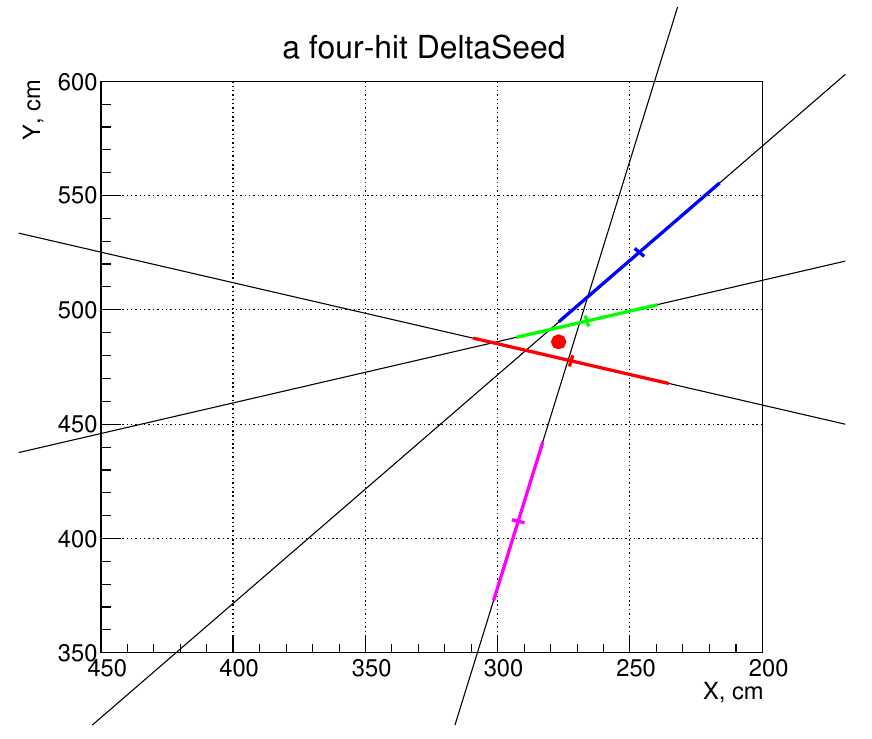
\includegraphics[width =0.6\textwidth]{figures/png/Screenshot_20240811_115854.png}
    \caption[]{    }
    \label{fig:deltaseeds}
\end{figure}
\paragraph{Step 2: Connecting Seeds}
DeltaFinder then connects segments close in both the $x-y$ plane and 
time across different stations to form $\delta$-electron candidates. 
A valid candidate must have at least two segments and a minimum of five straw hits. 
Reconstructed segments of a 100 MeV electron typically remain unconnected 
due to their separation in the $x-y$ plane.
DeltaFinder links $\delta$-electron seeds across stations, attempting to 
associate new seeds with existing $\delta$ candidates. If no match is found, a new candidate is created.
Good $\delta$ candidates are marked, and their hits are flagged 
to avoid their inclusion in proton candidate searches.


\paragraph{Step 3: Identifying proton candidates}
Finally, DeltaFinder identifies proton candidates by clustering high-ionization 
hits in time. The algorithm resolves overlaps between proton candidates and 
merges those with consistent segments across stations.

\iffalse

One of the central challenges of Mu2e is the reconstruction of conversion electrons in the face of
large amounts of backgrounds from other known processes that follow muon capture by the
aluminum atoms. The detailed background rates for these processes at this energy scale are not very
well studied. In Mu2e, background rates calculated according to figures given in Nuclear Physics of
Muon Capture (D. F. Measday) are used to create simulations. However, due to the lack of
documentation at the energy scales involved in this experiment, there is a large uncertainty in
background rates which requires background removal to be insensitive to the level of backgrounds
This primary purpose of study is to address one prevalent source of background hits: the
secondary ionized electrons, which are referred to as "deltas." Deltas consist primarily of Compton
scattered electrons, pair production electrons, and delta rays, in order of decreasing prevalence.
Compton scattered electrons are produced when photons from various processes strike material
inside the detector. This causes the ejection of electrons that create the background events. The
photons primarily originate from neutron capture by atoms, which leads to an excited nuclear state
that decays via photon emission. These photons generally have energies on the order of a few MeV.
The neutrons, in turn, are created when muons are captured by atoms, creating unstable isotopes that
decay by ejecting neutrons. Pair production electrons, on the other hand, are produced when
processes involving nuclear recoil also produce pairs of electrons and positrons in order to conserve
energy and momentum. Delta rays, or secondary ionized electrons, are produced when charged
energetic particles collide with detector material.






DELTAFINDER:
step 1: Find $\delta$-electron track segments separately within each station
connect segments, allow 1 station wide "gaps"
dominant sources of failures:
I stations with MC particle producing hits in only one face;
I hits with wrong coordinates along the wire - long tails of the $\Delta$T distribution;
I recover hits in "empty" stations to improve efficiency;
I optimization of the algorithm timing performance;
electron hit energy dependence on momentum: path length within the straw depends on momentum
only about 4\% of CE hits have energies above 3.5keV (1\% above 5 keV)
consider several hit energy cutoffs: 3.5 keV, 5keV, 7keV, use all hits




\subsection{Delta electron features}








Figure 2.1 shows the momentum distribution of deltas for 10,000 events.
Most deltas have much lower momenta than conversion electrons. This produces a significant
difference in their trajectories through the tracker, as shown in Figures 2.2 to 2.4. With the naked eye
one can already see dramatic differences.
The most striking quality of deltas is that they tend to create small, dense clusters of hits, as
shown in Figures 2.3 and 2.4. This motivates a "clustering approach"*: we search for such
concentrated clusters in the x-y plane using a clustering algorithm since deltas are very likely to reside
in such a cluster. However, the reverse containment does not hold - clusters can also contain many
conversion electron hits. Removing conversion electron hits can severely harm subsequent
reconstruction, so a filter is necessary. 
low energy (delta, compton, photon conversion) electrons are the largest source of the hits
in the tracker - about 2/3 of the total
language: $\delta$-electron - an electron with P<20 MeV/c
radius of a 10 MeV/c electron in the nominal Mu2e field < 3 cm, close to the resolution
along the wire
very specific topology - multiple hits with the same (X,Y) , within the resolution
\fi